\chapter{Application of \& \library{dEchorate}}\label{chap:ch:dechorate}

\openepigraph{Signal, a function that conveys information about a phenomenon.
$[\dots]$ Consider an acoustic wave, which can convey acoustic or music information.}{R. Priemer, \textit{Introductory Signal Processing}}
\vspace{-2.5em}

\section{Using the Data}
In this section we exemplify the utilization of the database considering three possible use-cases: acoustic echo estimation, echo-aware beamforming and room geometry estimation.

\subsection{Acoustic Echo Estimation}
\textit{Work in progress:
Use BSN, Crocco and BLASTER for echo acoustic echo retrieval.
\\Data: Sym/Real on Dirac/Noise/Speech}


\subsection{Echo-aware Beamforming}

\begin{figure}[h]
    \centering
    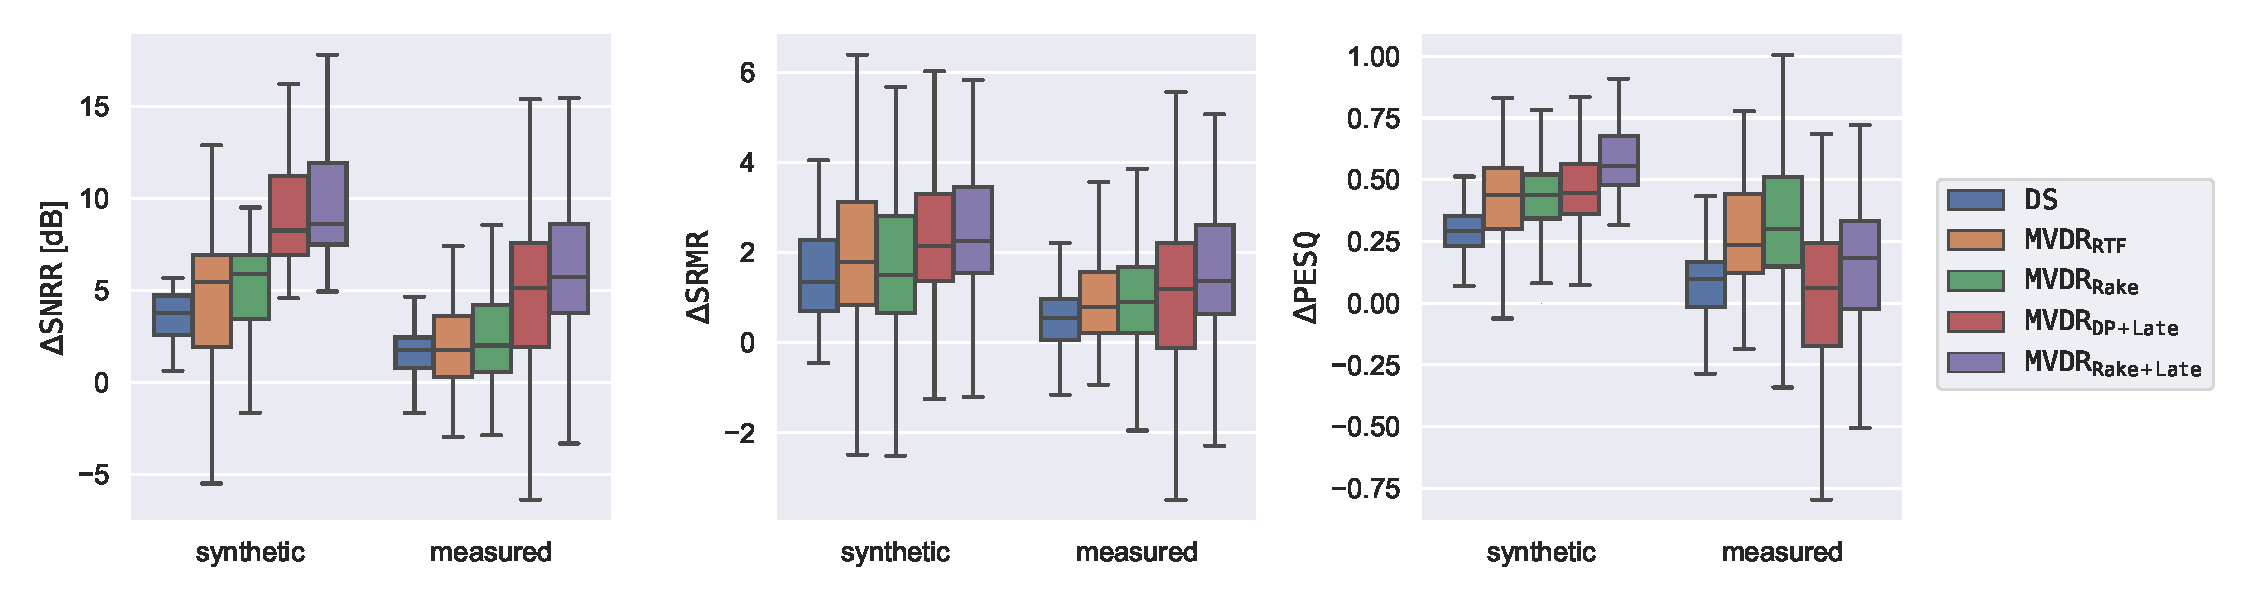
\includegraphics[trim={0 10 10 0},clip,width=\linewidth]
    {figures/dechorate/kowalkzy_results_boxplot.pdf}
    \caption{
    Comparison of echo-aware beamforming for the room configuration $\mathtt{011111}$ ($\RT \approx 600 $ ms) on measured and synthetic data  for all combinations of source-array positions in the \dEchorate{} dataset.}
    \label{fig:pesq}
\end{figure}

As mentioned, the knowledge of early echoes should boost spatial filtering performances. However the perfect knowledge of such elements are of difficult estimation. To investigate this, we compare two types of spatial filters on both synthetic and measured data: echo-agnostic and echo-aware beamformers.
\\The formers do not need any echo-estimation step: they either ignore their contributions, such in the direct-path delay-and-sum beamformer ($\DS$)~\citeonly{VanTrees2004Optimum}, or they consider coupling filters between pairs of microphones, called Relative Transfer Functions (RTFs)~\citeonly{gannot2001signal}\footnote{Note that, as opposed to AER, estimating the RTF is a non-blind problem.}.
The RTFs can be naturally incorporated in powerful beamforming algorithms achieving speech dereverberation and noise reduction in static~\citeonly{Schwartz2014multi}
and dynamic scenarios~\citeonly{Kodrasi2017evd}.
In this work, generalized eigenvector decomposition (GEVD) was used for the RTFs estimation~\citeonly{doclo2003robust}.
\\Echo-aware beamformers fall in the category of \textit{rake receivers}, borrowing the idea from telecommunication where an antenna rakes (\textit{i.e.} combines) coherent signals arriving from different propagation paths.
In particular, they consider ``partial steering vectors'' using known $R$ echoes' delays and attenuations~\citeonly{Jan1995matched}. This methods have been used for interfer and noise suppression in~\citeonly{Dockmanic2015raking} and for noise and reverberation reduction~\citeonly{Javed2016spherical, Kowalczyk2019raking}. Here we assume that echoes are known, computed from the geometry as in Section~\ref{sec:annotation}.

In addition to the standard $\DS$ design, we considered the minimum-variance-distrortionless-response design
echo-agnostic $\MVDR_\mathtt{RTF}$ build on RTFs as in~\citeonly{Schwartz2014multi} as echo-agnostic method, and the echo-aware beamformers $\MVDR_\mathtt{Rake}$~\citeonly{Dockmanic2015raking} and its extension for dereverberation, the $\MVDR_\mathtt{Rake+Late}$~\citeonly{Kowalczyk2019raking} considers the statistical contribution of the reverberation tail.

The performances of the different designs are compared for enhancing a target speech in 5-channel mixture (that is, one linear array used in the dataset) featuring high reverberation and diffuse babble noise, opportunely scaled to given signal-to-noise  ratio ($\SNR \in \kbrace{0, 10, 20}$).
Using the \dEchorate{} data, we considered the room configuration $\mathtt{011111}$ ($\RT \approx 600 $ ms) and all the possible combinations of target/array's positions. Both real and matching synthetic RIRs are used which are then convolved with anechoic speech from the WSJ corpus and corrupted by recorded diffuse noise.

The evaluation is conducted similarly to the one in~\citeonly{Kowalczyk2019raking}. We considered the following metrics: the signal-to-noise-plus-reverberation improvment (\DSNRR) in [dB] computed as difference between the input ($\mathtt{SNRR}$) at the reference microphone and the $\mathtt{SNRR}$ at the filter output; the speech-to-reverberation-energy-modulation ratio improvement (\DSRMR)\citeonly{falk2010non} as measure of dereverberation; and the perceptual quality of the signal is evaluated using the PESQ score.
As target signal, the clean signal convolved with the early part of the RIR (up to the $R$-th echo) is considered.
\\Numerical results are reported in Figure~\ref{fig:pesq}.
The simple $\DS$ beamformer is outperformed by the other filters, since more information is used to reduce noise and late reverberation.
When using synthetic data, the know echoes perfectly match numerically the components in the simulated RIRs. In this ideal scenario, one can see that the more information used the better the performances: RTF- and Rake- beamformers outperform the simple $\DS$ design; and including the late reverberation statistics boosts considerably all the performances.
Interestingly RTF-based design performs similarly to the Rake-one. This can be explained by the fact that GEVD method tends to robustly consider the stronger and more stable components of the RTFs, which in reverberant and noisy static scenario's are similar to the earlier portion of the RIRs.
\\When it comes to measured RIRs, the little errors in echo estimation, due to calibration mismatch, lead to a drop in the performances. This is even more clear when considering the $\dPESQ$ metrics, as it accounts also for artifacts. Here the echo-agnostic $\MVDR_\mathtt{RTF}$ outperform the other methods.


\begin{tabular}{c|cc|cc|cc|cc}
\toprule
source id &	1	& &	2	& &	3	& &	4 &	\\
wall &	DE&	AE&	DE&	AE&	DE&	AE&	DE&	AE\\
\hline
west &	0.74	& $\ang{8.99}$      & 4.59	& $\ang{8.32}$  & 5.89	& $\ang{5.75}$	& $\mathbf{0.05}$    & $\mathbf{\ang{2.40}}$\\
east &	$\mathbf{0.81}$	& $\mathbf{\ang{0.08}}$      & 0.9	& $\ang{0.50}$	&$\mathit{69.51}$	& $\mathit{\ang{55.70}}$	& 0.31    & $\ang{0.21}$\\
south&	3.94	&$\ang{16.08}$      & $\mathbf{0.18}$	& $\ang{1.77}$	&$\mathit{14.37}$ & $\mathit{\ang{18.55}}$	& 0.82    & $\mathbf{\ang{1.65}}$\\
north&	1.34	& $\ang{0.76}$	    & 1.40	& $\ang{8.94}$	& $\mathbf{0.63}$	& $\mathbf{\ang{0.17}}$	& 2.08    & $\ang{1.38}$\\
floor&	$\mathbf{5.19}$	& $\mathbf{\ang{1.76}}$	    & 7.27	& $\ang{2.66}$	& 7.11	& $\ang{2.02}$	& 5.22    & $\ang{1.90}$\\
ceiling&1.16	& $\ang{0.28}$	    & 0.67	& $\ang{0.76}$	& $\mathbf{0.24}$	& $\ang{1.16}$	& $0.48$    & $\mathbf{\ang{0.26}}$\\

\bottomrule
\end{tabular}

\subsection{Room Geometry Estimation}
The shape of a convex room can be estimated knowing the positions of first-order image sources. Several methods have been proposed which take into account different levels of prior information and noise (see~\citeonly{remaggi2016acoustic, Crocco2018room} for a review). Nonetheless, when the echoes' TOA and their labeling are known for 4 non-coplanar microphones, one can perform this task using simple geometrical reasoning as in \citeonly{Dokmanic2013acoustic}. In fact, the 3D coordinates of each image source can be retrieved solving a multilateration problem \citeonly{Beck2008ExactProblems} and the position and orientation of each wall can be easily derived from the ISM equations as the plane bisecting the line joining the real source position and the position of its corresponding image (see Figure~\ref{fig:wall_rec})

In \dEchorate{} the annotation of all the first order images for all the sound sources are available. Table~\ref{tab:res_rooge} shows the results of the estimation of the wall positions in terms of distance error (in centimeters) and surface orientation error (in degrees) using the four direct sources and all the 30 microphones, namely the 6 arrays). The room facets are estimated using each of the source as a probe. Despite few outliers, the majority of the facets are estimated correctly in terms of their placement and orientation with respect to the coordinate system computed in Section~\ref{sec:annotation}: for instance, for the source $\#4$, all 6 surfaces were localized with less than $6$ cm and $\ang{2.5}$ errors. Small errors are due to concurrency of multiple factors, such as tiny offsets in the annotation and the ideal shoebox approximation. In the real recording room, some gaps were present between revolving panels in the walls. In addition it is possible that for some source-receiver pairs the far-field assumption is not verified, causing the inaccuracy of \textit{reverting} the ISM. Finally, the 2 outliers for the source $\#3$ are due to a wrong annotation caused by source directivity and mis-classification. When a wall is ``behind'' the source, the energy of the related $1^\text{st}$ reflection is very small and might not appear in the RIRs. This happened for the eastern wall and a second order image was taken instead. Secondly, the contribution of multiple reflections arriving at the same time can results in large late spikes in estimated RIRs. This effect is particularly amplified when the microphone and loudspeakers exhibit long impulse responses. As a consequence, some spikes can be miss-classified. This happened for the southern-wall were again a second-order image was taken instead. Nevertheless, this second type of errors can be manually corrected and the annotations updated.

% \begin{figure}[h]
%     \subfigure{
%         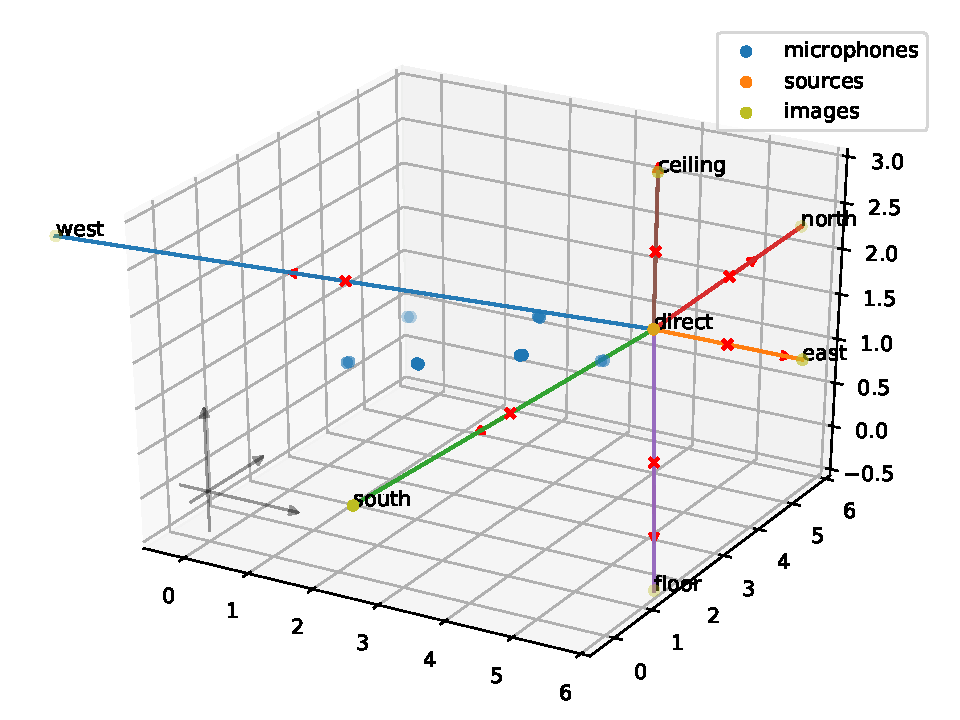
\includegraphics[width=0.49\textwidth]{figures/estimated_image}}
%     \hfill
%     \subfigure{
%         \includegraphics[width=0.49\textwidth]{figures/estimated_reflector}}

%     \caption{Images source estimation (right) and corresponding reflector estimation (left) for one of the sound sources in the dataset.}
%     \label{fig:wall_rec}
% \end{figure}

\begin{figure}

        \includegraphics[width=\linewidth]{figures/dechorate/estimated_reflector}

    \caption{Images source estimation and reflector estimation for one of the sound sources in the dataset.}
    \label{fig:wall_rec}
\end{figure}

\section{Conclusions and Perspectives}

This paper introduced a new database of room impulse responses featuring accurate annotation of early echoes and microphone positions. These data can be used to test methods in the room geometry estimation pipeline and in echo-aware audio signal processing. In particular, robustness of these methods can be validated against different levels of $\RT$, SNR or even early echo density.